\chapter*{Introduction}\label{chap:intro}
\addcontentsline{toc}{chapter}{Introduction}
\chaptermark{Introduction}

When answering the classic question ``What is your Ph.D. about?'' to family and friends, I always start with the ``Ctrl + F'' function in their favorite text editor or web browser. This quickly highlights one of the applications of the exact pattern-matching problem. If I feel especially ambitious in my explanations, I will attempt to give the intuition of the naive $\Oh(nm)$ algorithm. Picture a young child, aligning the string against every position of the text and comparing character by character because the child has yet to learn how to read. To give a glimpse at a more complex solution, I comment on how, depending on the word, the child may try to skip portions of the text. But even my grandparents immediately know that searching in a text has been possible for decades and that it cannot be my real research subject.

\section{Context}

Indeed, exact pattern matching has been long studied, with in particular the famous Knuth-Morris-Pratt algorithm\footnote{The elegance of this algorithm is what first drew me in this area of research as a bachelor student!} published in 1977~\cite{KMP} after being independently discovered by Morris-Pratt in a technical report in 1970 and Knuth in 1973. Since then, this has become one of the classic textbook algorithms, and Charras and Lecroq published a detailed handbook~\cite{charras2004handbook} on the various solutions to exact pattern matching.

\subsection{Complex exact queries} 

% Define center type column
\newcolumntype{Y}{>{\centering\arraybackslash}X}
\newcolumntype{P}[1]{>{\centering\arraybackslash}m{#1}}
\renewcommand\tabularxcolumn[1]{m{#1}}

%spacing
\renewcommand{\arraystretch}{2}
\begin{figure}[h]
    \begin{tabularx}{\textwidth}{P{3cm} P{4.5cm}  Y }
        Matching model & Pattern & Text with occurences underlined \\
        \hline
        Regular Expression~\cite{RM-704} & $P=$ GAT$(\mathrm{TA}\mid \mathrm{O})(\mathrm{CAT})^*$ & $T=$ \underline{GATTA}AT\underline{GATOCATCATCATCAT}A \\
        Error bound~\cite{landau1986efficient} (for ED~\cite{levenshtein1966binary}) & $P=$ GATTACAT & $T=$ AT\underline{GATTAACAT}ATA, $\mathrm{ED}(P,T[2..10])=1$ \\
        Don't care~\cite{fischer1974string} & $P=$ GAT**CAT & \underline{GATTACAT}A\underline{GATOACAT}AC\\
        %
        Gapped consecutive~\cite{bille2022gapped} & $P_1=$ GATTA $P_2=$ TAC  $a=2$, $b=6$ & $T=$ AGG\underline{GATTAC}TAC, $d=3 \in [a,b]$\\
        %
        Elastic Degenerate~\cite{iliopoulos2021efficient}  & $P=$ GATTACAT &  $T=$ {\renewcommand{\arraystretch}{1} AT\underline{GAT}$\left\{
            \begin{array}{l}
                \mathrm{\underline{TA}}  \\
                \mathrm{O}
            \end{array}\right\} \mathrm{\underline{CAT}A}$} \\
        %
        Abelian/Jumbled~\cite{eres2004permutation} & $P=$ GATTACAT & $T=$ AGAG\underline{TATGATC}AGT\\
        %
        Order preserving & $P =$ 1 5 3 4 6 2 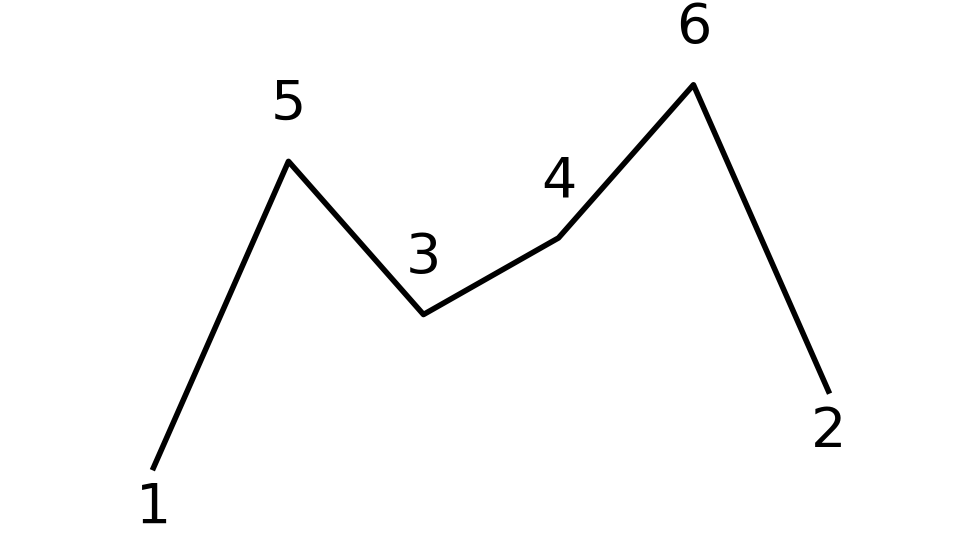
\includegraphics[width=3.5cm]{Introduction/op_P.png} & $T=$ \underline{2 7 4 5 8 3} \underline{1 20 15 16 25 6}  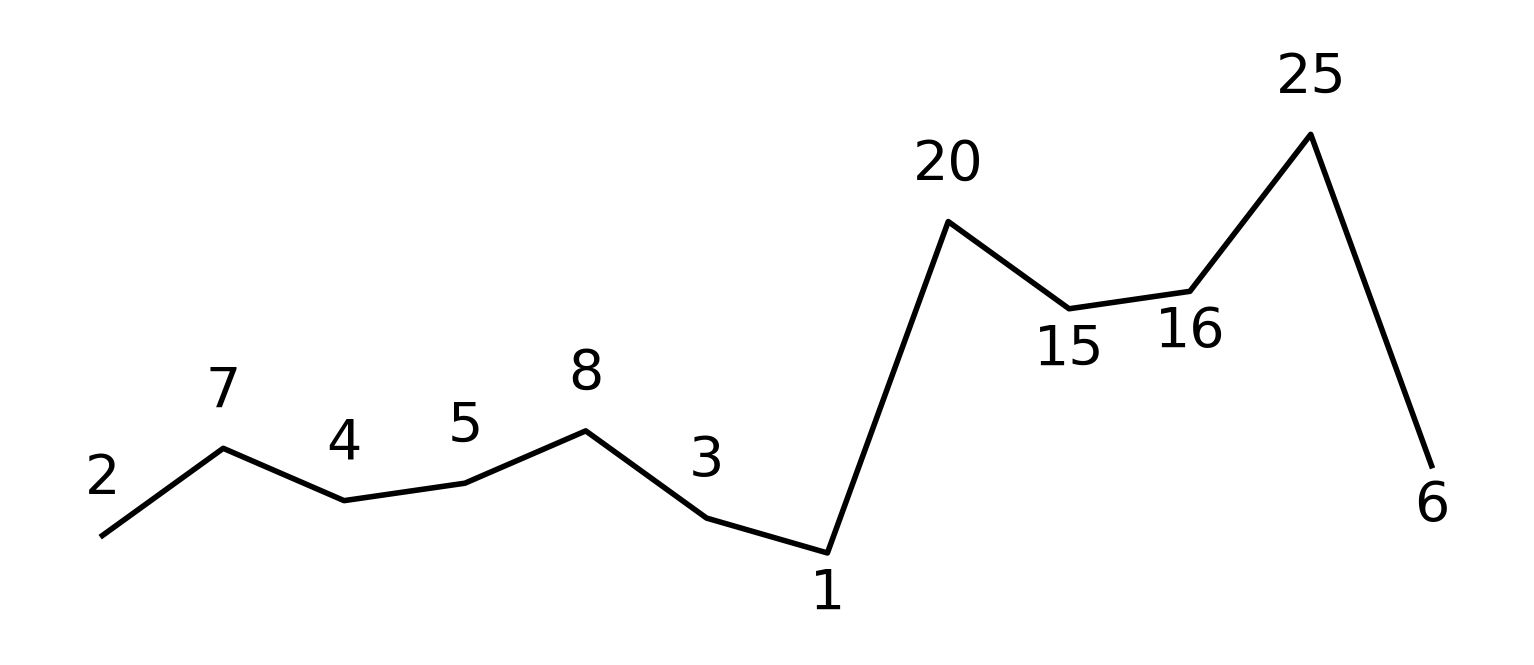
\includegraphics[width=5cm]{Introduction/op_T.png} \\
        %
        Parametrized~\cite{baker1993theory} & $P=$ GATTACAT & $T=$ OPO\underline{POGGODOG}O, {\footnotesize A:O, C:D, G:P, T:G} \\
    \end{tabularx}
    \caption{Example of various model of matching on strings.}
    \label{fig:intro:match_model}
\end{figure}

However, the need for text processing goes far beyond exact matching of patterns. To illustrate this claim, we present the models of matching considered in this manuscript and their motivations. Figure~\ref{fig:intro:match_model} also provides an example for each matching model.


\todo[inline]{Detail Regular expression much more}
% Regular expression
One of the oldest and most classic models for more complex queries is \underline{regular expressions} introduced by Kleene in 1951~\cite{RM-704}.
% Briefly explain the formalism
The regular expression formalism provides a concise representation for defining sets of strings by recursively employing three fundamental operators: concatenation, union, and Kleene star.
% Application and Limitations
It has deep connections with automatons~\cite{Thompson_automaton}, and its versatile nature makes it a crucial tool in many fields such as internet traffic analysis~\cite{4221791,4579527}, databases, data mining~\cite{1000341,10.5555/645927.672035,10.1145/375551.375569}, computer networks~\cite{10.1145/1159913.1159952}, and protein search~\cite{10.1145/369133.369220}. Chapter~\ref{chap:regexp} provides a new streaming algorithm for regular expression membership and pattern matching.

 \todo[inline]{Detail and have a better transition for don't care}

% Don't care
As an alternative, Fischer and Paterson~\cite{fischer1974string} introduced \underline{``don't care''} matching where a don't care symbol denoted * can occur in both the pattern and the text, matches to any other character of the alphabet (but only one).
% Gapped matching
\todo[inline]{Add a more general review of models where one or two patterns are search spaced at a certain distance}
The ``don't care'' matching model is sometimes referred to as ``gapped'' matching; however, it is not to be confused with \underline{gapped consecutive matching}~\cite{bille2022gapped} where we are given two patterns $P_1$ and $P_2$ as well as an interval $[a,b]$ and must report all occurrences of $P_1$ and $P_2$ with the distance in $[a,b]$ and no occurrences in between. This model also has connections to spaced seeds~\cite{burkhardt2003better}, and we study it in various settings in Chapter~\ref{chap:gapped_stream}, ~\ref{chap:gapped_pm} and~\ref{chap:gapped_index}.


Although an in depth non-standard matching listing is out of the scope of this manuscript, for completeness, we detail other models of the literature.
% Degenerate strings
The modelization of flexible and diverse DNA sequences~\cite{comm1970iupac} lead to the model of \underline{degenerate} strings~\cite{abrahamson1987generalized} (also called indeterminate) where each position of the string corresponds to a subset of $\Sigma$.
% (Elastic/Generalised) Degenerate strings
This model has recently been continued in two directions: \underline{elastic degenerate} strings~\cite{iliopoulos2021efficient} where each position is a subset of strings over $\Sigma$ and \underline{generalised degenerate} strings~\cite{alzamel_et_al:LIPIcs:2018:9323} where each position is a subset of strings of $\Sigma^k$ but where the length $k$ can vary from position to position.
%\todo{Detail the biological problem behind the model}
% Weighted string
Alternatively, when probabilities are given for each character and positions in the form of a position weight matrix~\cite{thompson1994clustal} the strings are called \underline{weighted} (or uncertain). Then, the cumulative probability that a string occurs at a starting position is the product of the probabilities of the corresponding character at each position.
% Abelian/jumbled/many other names 
In the model of \underline{abelian} matching, a string (or a substring) is entirely identified by the letter it contains (with multiplicities), disregarding their order. It stems from the automatic discovery of clusters of genes in genomes where they can occur in a different order but still linked to the same function~\cite{eres2004permutation}, but the same concept has also been used in the context  of using mass spectrometry for DNA assembly~\cite{bocker2003sequencing} where the strings without order are called compomers. This model is also known as jumbled, permutation, and many other names, and Tahir Ejaz dedicated his thesis~\cite{ejaz2010abelian} to this model.
% order preserving
The \underline{order-preserving} model~\cite{kim2014order,kubica2013linear} takes a somewhat opposite approach and says that two strings match if they have the same relative shape: $\forall i,j \in [0,n-1], X[i] < X[j] \leftrightarrow Y[i] < Y[j]$. This matching model aims at capturing the trend detection needed in the stock market and music melody matching problems~\cite{kim2014order}.
%
% Parametrized matching
Another application-driven model is \underline{parametrized strings} or ``p-string'' introduced by Baker~\cite{baker1993theory}, where two strings match if we can transform one into the other by applying a one-to-tone function renaming the parameters, meant to detect code duplication.

\subsection{Repetition detection}
\todo[inline]{Work in progress do not review!\\ TODO: Detail}
So far we focussed on matching models where we are given a pattern and text as well as conditions that define a match of the pattern in the text. But another central task in text processing is repetitions detection. By repetitions, we refer to consecutive occurrences of the same fragment. They can be repeated twice (a square), three times (a cube) or more, then represented as a run: a maximal periodic substring. They are needed as a theoretical tool to avoid needless repetitive computations, but they also naturally occur in DNA with an important role in genomic fingerprinting~\cite{Kolpakov2003}.
The study of squares in strings goes back to 1906 with the work of Thue~\cite{thue1906} on the construction of an infinite square free word, in Chapter~\ref{chap:squares} we provide an optimal algorithm for square detection.


\subsection{Approximate queries}
\todo[inline]{Work in progress do not review!\\ TODO: Complete rewrite and add citations about other model with mismatches}
% Similarity measures & approximate matching
Although regular expressions are powerful, Bioinformatics\cite{Gusfield1997}, music analysis~\cite{mongeau1990comparison} and plagiarism detection~\cite{lukashenko2007computer} also need relevant and efficient similarity measures such as the Levenshtein distance~\cite{levenshtein1966binary} or Dynamic Time warping distance~\cite{sakoe1978dynamic}. They also often need to report all occurrences with an error bound\cite{landau1986efficient,landau1989fast}: at a distance at most a threshold $\tau$.
We contribute to this line of research in Chapters~\ref{chap:LCS} and~\ref{chap:DTW}.


\subsection{Scalability Issues}

%%%%%%%%%%%%%%%%%%%%%% Intro scalibility %%%%%%%%%%%%%%%%%%%%%%%%%%%%
 
% But it is not just about the specific model also about scalibility
We discussed so far how string processing tasks have crucial industry-relevant applications, but another major challenge in most applications is the scalability to large datasets.
% Wikipedia
Highly curated datasets generally remain quite small, for example the English pages of Wikipedia (just the text and metadata) take up 20~gigabytes in a compressed format as of 2022~\cite{wikimedia}. In comparison, any form of archival and version history tends to grow much bigger. Just the metadata of revision's history (without the content of the articles) for the Wikipedia English pages takes up 75~gigabytes still as of 2022.
% Software Heritage
It is sometimes possible to limit the redundancy in the archive data, for example by using a graph which tracks where the data is repeated multiple times. This is the approach taken by the Software Heritage~\cite{swh-site} project, which aims at keeping an archive of entirety of the software code produced by humanity. The graph structure is especially necessary in this project to reduce code redundancy and reflect the standard use of version history management in software development.
Substantial research and engineering effort~\cite{DBLP:phd/hal/Pietri21} were made to provide an efficient navigation of the graph. 
However, since the code repositories are indexed based on their URLs and metadata, it is not currently feasible to perform a search specifically for occurrences of a particular code snippet\footnote{\setlength\parindent{10pt} A silly but interesting example is~\cite{vii2014if} where the author searched \texttt{"const double epsilon ="} (and equivalents in other \par languages) on all GitHub repositories to study the value programmers typically chose for epsilon.}.
As of 2023, the graph is limited to 7~terabytes but with the source files the space usage approaches 1~petabyte~\cite{swh-polytechnique}.
% Internet archive
Another example of a large archival project is the internet archive, a non-profit which started saving web pages in 1996 and now holds the history of more than 800 billion web pages through their program: the wayback machine~\cite{web-archive}. This archive takes up more than 70~petabytes, however, one of the limitations is that the search options are limited to the metadata of the websites and not the content of the webpages themselves.


%%%%%%%%%% Bioinformatics
%Intro DNA representation
Large archival also exist in bioinformatics, but the structure of biological sequences is very different from the one of code or webpages.
DNA is most commonly seen as a string over the nucleotide alphabet \texttt{\{A,T,C,G\}} which can be stored using just 2 bits per base. However, this type of storage does not provide fast queries. 
At the opposite of the spectrum, a suffix tree allows efficient sequence analysis but requires 10 bytes per base~\cite{navarro2016compact}, which adds up to 30 gigabytes for a human genome containing 3.3 billion bases.
A trade-off between those two extremes has been found through the development of compact data structures that exploit redundancy to decrease space usage. For a human genome it allows to represent the sequence and its suffix tree using just 4 gigabytes~\cite{navarro2016compact}. 
% Reads
However, for DNA, another classic data model is the one of reads: when DNA is sequenced, the output is a set of fragments (called \emph{reads}) of the original sequence. Reads can contain sequencing errors such as insertions, deletion and substitution of a nucleotide and their length and error rate vary depending on the sequencing techniques. To be able to reconstruct the original sequence, reads are extracted in such quantities that each base is covered multiple times. This means readsets are larger than the assembled genome and even more redundant. In Chapter~\ref{chap:XBWT} we explore this topic for Illumina reads and propose a data structure specifically tailored to sequencing technique's specificities. 
% Cheaper = more sequencing
Additionally, drastic decrease in sequencing cost since 2008 (faster than expected by Moore's law~\cite{muir2016real}) lead higher volumes of DNA being sequenced. 
% ENA
So far, the European Nucleotide Archive has accumulated more than 47 petabytes\cite{ena} of read data.
% SRA
While the NCBI Sequence Read Archive has more than 73 petabases~\cite{sra} of archive including 38 petabases in open access. Again, in those datasets the data is indexed by its metadata only.\\
%\todo[inline]{Look for more reasonable size example ? It's unclear if anybody would want to index the entire SRA}

%%%% Astronomical data 
\todo[inline]{Add applications to astronomical data and pulsar detection.}
\todo[inline]{Add one or several graphs illustrating the growth in data in each field.}

%%%%%%%%%%%%%%%%%%%%%% Approaches to adress scalibility %%%%%%%%%%%%%%%%%%%%%%%%%%%%
\todo[inline]{Introduce the concept of sketches and then add to each approach to scalability how it interacts with sketches (for the title of the PhD).}
It goes without saying that algorithms with quadratic time complexity cannot scale to terabytes and petabytes of inputs. Consequently, the choice of query is dictated by the specific needs of the application and the typical scale of the input.
Several (overlapping) approaches are generally used to cope with large amounts of data:
\begin{itemize}

\item Distributed algorithms: those are designed to work on several computers sharing a network. The data is processed in parallel with limited transfer over the network (those transfers can be 10 times slower compared to disk transfer). This direction is a research field of its own which is out of the scope of this thesis.
\item Compressed input: as mentioned several times already, highly redundant data can sometimes be compressed to a manageable size. 
Consequently, algorithms and data structures that can directly operate on the compressed data become much more efficient. This is very natural approach as the data is almost always shared in a compressed format, however not all problems can be solved faster with this approach. For example, Abboud et al.~\cite{abboud2017fine} showed that for computing the longest common subsequence of two strings of uncompressed size $N$, given in a compressed format of size $n$, there is a lower bound $(nN)^{1-o(1)}$ assuming the strong exponential time hypothesis. In other words, even if the input is given compressed form, we cannot avoid a high dependency in the uncompressed size. In this thesis, 
chapters~\ref{chap:gapped_pm} and~\ref{chap:gapped_index} both work on a grammar compressed text.
\item Data structures: here the complexity analysis is split in two parts, the \emph{construction} and the \emph{query}. The construction is generally more expensive and meant to be performed once, whereas the queries are meant to be fast and performed multiple times with varying input-query. The size of the data structure refers to the space of the information kept at the end of the construction to perform the query.   
%One of the use case is to construct on a powerful server and then send the small data structure to users that can loaded it in main memory and query it repeatedly. 
Chapters~\ref{chap:gapped_index} and ~\ref{chap:XBWT} are examples of that.
\item Efficient second-memory algorithms: One of the challenges when dealing with large inputs is the quantity of main memory used, as most computers are still limited to gigabytes of RAM. To circumvent this limitation, programs may resort to working directly from secondary memory as disk space scales at a much cheaper cost than RAM.
It is  common knowledge that random access to disk is very inefficient, however contiguous reads are only 100 time slower than reading from main memory~\cite{navarro2016compact}. Therefore, an algorithm that uses few random reads can be executed directly on disk which allows it to scale to large inputs much more easily. The main issue with this approach is that not all problems can avoid random access. We partially use this approach to limit main memory usage in chapter~\ref{chap:XBWT}. The construction of the index is split in phases that read contiguously from disk, process the information (for the next phase or final output) and write to disk.
\item Streaming algorithms: if the data is so large that it can only be handled as a stream, then it must be processed on the fly without the possibility to go back. Generally the pattern and the length of the text are known in advance and can be preprocessed, then the characters arrive one by one and can only be accessed later if they have been explicitly stored. This model optimizes for both the time per character during the streaming phase and the space complexity which accounts for storing the result of the preprocessing and any space necessary to process the characters. Chapter~\ref{chap:regexp} and~\ref{chap:gapped_stream} are set in this model.
\item Approximation algorithms: On a very large dataset it is not always needed to answer queries exactly and allowing some approximation in the result can allow to cut corners and circumvent lower bounds. The entire second section of this thesis is related to this approach but Chapter~\ref{chap:LCS} is perhaps most characteristic. We treat the problem of the Longest Common Subsequence with approximately $k$ mismatches with a probabilistic algorithm that answer correctly with high probability. %($\geq 1 - \frac{1}{n}$ for an input of size $n$).
\end{itemize}

\section{Contributions}\label{intro:sec:contrib}

So far, we presented the two core challenges at the heart of text processing: enabling relevant (and sometimes complex) queries suited to specific applications and while maintaining performances that can scale to the large volumes of input data.
%
This thesis makes theoretical and practical contributions to address both needs. 
Each contribution is presented as an independent chapter corresponding to a publication. This choice was motivated by the variety of subjects and techniques as well as how they were conceived as independent projects (with varying sets of co-authors) during the Ph.D. This section is meant to give an overview of the main contributions of the thesis and how they relate.

\todo[inline]{Extend the abstract description of how the different project relate to each other.}
